\section{Verschlüsselung}
Kryptographische Schlüssel werden von dem Betriebsystem für die Ver- und Entschlüsselung von 
Informationen verwendet. Daten werden verschlüsselt, um die darin enthaltenden Informationen 
vor potentielle Angreifer geheimzuhalten. Die Verschlüsselung von Daten kann vielfältig eingesetzt 
werden, typische Anwendungszwecke können bspw. die Verschlüsselung einzelner Dateien oder gar 
des gesamten internen Dateisystems sein. \cite{symmetricenc}


\subsection{Verschlüsselungalgorithmus}
Für die Verschlüsselung der Datenaustausches zwischen Komponenten, Systemen oder Apps
werden unter iOS unterschiedliche Varianten des etablierten Verschlüsselungsverfahrens
AES (Advanced Encryption Standard) eingesetzt. AES ist ein symmetrisches Verschlüsselungsverfahren,
die miteinander interagierenden Parteien müssen also einen gemeinsamen Schlüssel austauschen, welcher
daraufhin für das ver- und entschlüsseln von Informationen verwendet wird. \cite{symmetricenc} \cite{apple2020} \\

	\begin{figure}[h]
		\centering
		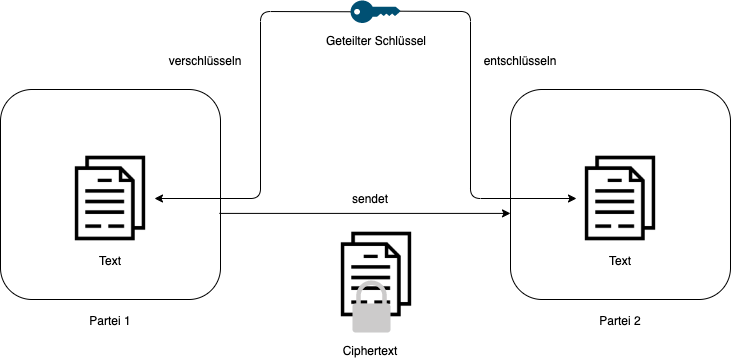
\includegraphics[width=135mm]{images/symmetric.png}
		\caption{Symmetrische Verschlüsselung \cite{symmetricenc}}
		\label{fig:symmetric}
	\end{figure}

\pagebreak

\subsection{Hardwaresicherheit}
Anhand der Beschreibung des symmetrischen Verschlüsselungsverfahren wird deutlich, dass die Schlüssel in
gesicherten Umgebung verwaltet und verwendet werden müssen. Anderenfalls kann nicht von der Vertraulichkeit 
der Daten ausgegangen werden, weil ein Angreifer möglicherweise durch den Diebstahl der Schlüssel den Datenverkehr
mitlesen kann. \cite{apple2020} \\

Aus diesem Grund werden in modern iOS-, iPadOS- und watchOS-Geräten Sicherheitschips verbaut, die einen sicheren
Coprozessor enhalten. Dieser Coprozessor wird auch \textit{Secure Enclave} genannt und ist ein hardwarebasierter 
Schlüsselmanager, der von dem Hauptprozessor isoliert ist. Dadurch wird eine weitere Sicherheitsebene in die 
Verwaltung der sicherheitskritischen Schlüssel umgesetzt. Die Verschlüsselungsschlüssel werden nicht mal
der CPU oder dem Kernel des Betriebsystemes offengelegt, weil diese potenziell von einem Angreifer manipuliert
werden können. Außerdem enthält der Sicherheitschip eine Hardware-AES-Engine, die für die Ver- und Entschlüsselung
von Dateien mithilfe des AES-Verschlüsselungsalgorithmus eingesetzt wird. Während des Start des Systemes tauschen
die Secure Enclave und die AES-Engine einen temporären Schlüssel miteinander aus. Mithilfe des temporären Schlüssels
können die beiden Komponenten sicher innerhalb des Sicherheitschips kommunizieren. \cite{apple2020hardware_security} \cite{apple2020} \\

\subsection{Schlüssel- und Passwörterverwaltung}
Sicherheitskritische Daten wie kryptographische Schlüssel oder Passwörter müssen in einer gesicherten Umgebung
verwaltet werden können. Mit der Secure Enclave wurde bereits eine Methode zum Speichern dieser Daten erläutert, 
in den folgenden Abschnitten werden weitere Methoden, die iOS und iPadOS verwenden, vorgestellt. \cite{apple2020}

\subsubsection{Schlüsselbund}
Mobile Anwendungen müssen oftmals vertrauliche Daten, wie bspw. Passwörter oder Tokens, auf dem Gerät hinterlegen. 
Das Betriebssystem bietet dafür den sogenannten Schlüsselbund an. Diese Komponente ist eine SQLite-Datenbank,
welche die sensiblen Daten in verschlüsselter Form speichert. Der Schlüsselbund befindet sich dabei \textbf{nicht} in der
Secure Enclave, sondern im Gerätespeicher. Dies ist aber dennoch sicher, weil der Verschlüsselungsschlüssel, welcher
für die Entschlüsselung der Daten benötigt wird, sich in der Secure Enclave befindet. \cite{apple2020}

\subsubsection{Zugriff auf den Schlüsselbund durch Apps}
Wie bereits erläutert, ist der Schlüsselbund durch eine verschlüsselte SQLite-Datenbank realisiert, die im Dateisystem hinterlegt ist. Eine App kann den Schlüsselbund verwenden um Passwörter, Kreditkarteninformationen, Zertifikate, Identitäten oder auch kurze Notizen verschlüsselt zu hinterlegen \cite{apple2020keychain_services}.
Diesen Daten können Attribute zugeordnet werden, welche nicht verschlüsselt sind, sodass die Daten auch nach der Verschlüsselung im Schlüsselbund gefunden werden können \cite{apple2020keychain_items}. 

\begin{figure}[h]
	\centering
  		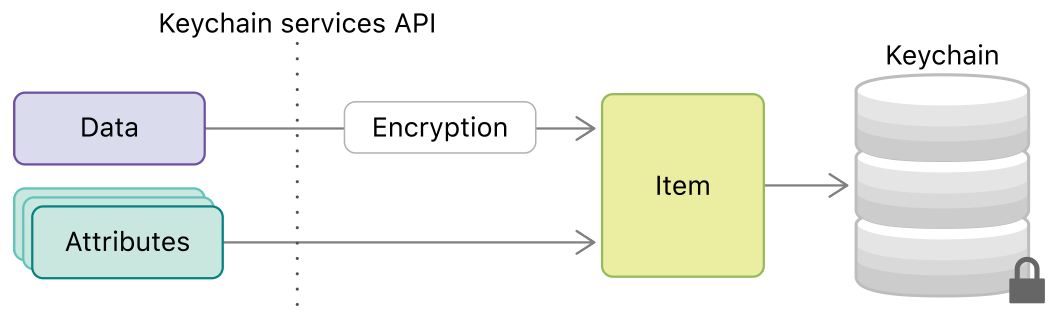
\includegraphics[width=1\textwidth]{../images/keychain-api-example}
		\caption{Hinzufügen eines Eintrags zu dem Schlüsselbund durch App \cite{apple2020keychain_items}}
		\label{fig:add-entry-to-keychain}
\end{figure}

Der Zugriff durch eine App auf den Schlüsselbund geschieht durch den \textit{securityd}-Daemon (Abb. \ref{fig:add-entry-to-keychain}). Dieser bietet eine API zum Speichern beziehungsweise Verschlüsseln und Auslesen von Schlüsselbundeinträgen. Zudem  entscheidet der Deamon auf Basis der Berechtigung \textit{keychain-access-groups}, welche App auf welchen Eintrag im Schlüsselbund zugreifen darf. Durch die Klassifizierung der Apps in Gruppen, können Informationen innerhalb dieser Gruppen ausgetauscht werden \cite{apple2020keychain_item_groups}. Somit muss ein*e Nutzer*in sich nur in einer von zwei oder mehr zusammenhängenden Apps authentifzieren und ist unmittelbar auch in den anderen der Gruppe zugehörigen Apps angemeldet. Als Voraussetzung gilt auch hier, dass die Apps von dem gleichen Entwickler*innenteam veröffentlicht wurden. \\
Apps die neben dem Schlüsselbund auch weitere Daten austauschen möchten, sind einer \textit{application-group} zugehörig.  Somit können gemeinsame Container verwendet oder durch eine Interprozesskommunikation Informationen ausgetauscht werden \cite{apple2020keychain_application_groups}. 


\subsubsection{Keybags}
Keybags sammeln und verwalten die Schlüssel der verschiedenen Datensicherheitsklassen. Jeder Keybag verwaltet aber
nur die Klassenschlüssel seines Types, im dem folgenden Kapitel werden diese vorgestellt und ihre 
Funktionsweise erklärt. \cite{apple2020}
Für die verschiedenen kryptografischen Verfahren, die bei der Gewährleistung von Sicherheit in iOS zur Anwendung kommen, werden Schlüssel benötigt. Diese werden in so genannten \textit{Keybags} abgelegt und können mit Hilfe des \textit{keybagd} Deamon ausgelesen und gespeichert werden.
Es gibt in iOS die fünf \textit{Keybags}, \textit{User}, \textit{Device}, \textit{Backup}, \textit{Escrow} und \textit{iCloud Backup}, die unter anderem auch bei den Datei- beziehungsweise  Schlüsselbund-Datensicherheitsklassen  zum Einsatz kommen.\cite{apple2020}

\paragraph{User}{Enthält alle normalen, für den Betrieb notwendigen, Klassenschlüssel und wird durch die \textit{Secure Enclave} verwaltet. Ein Zugriff ist erst nach erfolgreichem Entsperren des Gerätes möglich. }

\paragraph{Device}{Wird für das Speichern von Schlüsseln verwendet, die unabhängig von Benutzerkonten benötitgt werden.}

\paragraph{Backup}{Enthält die Schlüssel, die für das Erstellen eines verschlüsselten Backups durch iTunes auf einem Computer, notwendig sind. Dieser \textit{Keybag} wird durch ein Passwort gesichert, welches in iTunes festgelegt wird.}

\paragraph{Escrow}{Dieser \textit{Keybag} enthält Schlüssel für die Verbesserung der Benutzerfreundlichkeit beim Synchronisieren von Geräten. Dafür muss ein Gerät in einem ungesperrten Zustand mit iTunes verbunden werden, wodurch eine Paarung stattfindet, sodass der Gerätecode nicht erneut eingegeben werden muss. }

\paragraph{iCloud Backup}{Ermöglicht die gleiche Funktionsweise zum \textit{Keybag} \textit{Backup}, für die Realisierung eines Backups durch die iCloud. }


